%!TEX root = ../dokumentation.tex

\chapter{Gruppenarbeit}\label{cha:Gruppenarbeit}
Die Aufgabe bestand in der Implementierung einer 2003-Architektur. Da unsere Gruppe aus vier Mitgliedern besteht, wurde eine 2004-Architektur implementiert. Die Implementierte Anwendung
Für die Calculators haben wurde ein Interface entwickelt, welches jeder Calculator implementiert. Dieses Interface bietet eine Methode, um die Ergebnisse der Berechnungen der Calculators abzufragen.
Die Main-Klasse bildet den Einstiegspunkt des Programms und bündelt die Funktionalität zum Aufrufen der Calculators und der Voting-Funktionalität.

Für die Operatoren, die die Calculators unterstützen, wurde ein Enum-Datentyp erstellt

\section{Aufrufen der Calculators}
Zum Aufrufen der Calculators und Aufrufen des Votings wurde die Methode calculate entwickelt.

Diese hat eine Liste an CalculatorInput-Objekten als Eingabeparameter und erzeugt auf Grundlagen dessen vier Calculator-Objekte basierend Calculator1, Calculator2, Calculator3 und Calculator4. Diese vier Calculator-Objekte werden dann in eine List gefügt, um anschließend durch diese zu iterieren und die Methode getResult des Interfaces aufrufen. Die zurückgegebenen Ergebnisse der getResult-Methode werden in eine neue Liste gefügt. Mit den Ergebnissen wird die Vote-Methode aufgerufen.
Vor dem Aufruf der Voting-Funktionalität werden die Eingabedaten ausgegeben, damit das Voting-Ergebnis nachvollzogen werden kann.
Für jeden Fall (0 Fehler, 1 Fehler, …) wurde eine Methode erstellt, welche die calculate-Methode mit den korrespondierenden Eingabedaten aufruft.
\section{Voting}


\section{Implementierung der einzelnen Calculators}
Die Implementierung der Calculators ist in den folgenden Abschnitten beschrieben. Bei der Implementierung wurde darauf geachtet, dass nicht alle Calculators gleich implementiert sind, da dies dem Sinn der 2004-Architektur nicht entsprechen würde. Alle Calculators besitzen ihre eigenen Unit-Tests. 

\chapter{Calculator 1 (Bearbeiter: 8540946)}
\begin{lstlisting}[language=Java,basicstyle=\scriptsize, caption= Calculator 1]
public class Calculator1 implements ICalculator {
    private double _value1;
    private double _value2;
    private Operator _operator;

    public Calculator1(double value1, double value2, Operator Operator){
        this._value1 = value1;
        this._value2 = value2;
        this._operator = Operator;
    }

    @Override
    public double getResult() {
        double result = 0;
        switch (this._operator){
            case PLUS:
                result = add();
                break;
            case MINUS:
                result = subtract();
                break;
            case DIV:
                result = divide();
                break;
            case MULT:
                result = multiply();
                break;
        }
        return result;
    }

    private double add(){
        return this._value1 + this._value2;
    }

    private double subtract(){
        return this._value1 - this._value2;
    }

    private double divide(){
        return  this._value1 / this._value2;
    }

    private double multiply(){
        return this._value1 * this._value2;
    }
}
\end{lstlisting}
Die Klasse \textit{Calculator1} implementiert das Interface \textit{ICalculator} und besitzt drei Attribute vom Typ \textit{double}: \textit{\textunderscore value1}, \textit{\textunderscore value2} und \textit{\textunderscore operand}.\\
Dem Konstruktor der Klasse werden die Eingabeparameter value1, value2 und operand übergeben und dieser setzt die Klassenattribute gleich der Eingabeparameter.\\
Neben den drei Attributen besitzt die Klasse die vier private Methoden \textit{add()}, \textit{subtract()}, \textit{multiply()} und \textit{divide()}.
Diese sind Hilfsfunktionen, um aus den \textit{values} das Ergebnis zu berechnen.
Welche dieser Methoden aufgerufen wird, hängt von dem Operator ab.\\
Dieser wird geprüft, wenn der Nutzer die Methode \textit{getResult()} aufruft.
Die Methode \textit{getResult()} implementiert die entsprechende Methode des Interfaces.
Über die switch-Anweisung wird die zu dem jeweiligen Operator passende Methode zur Berechnung aufgerufen und am Ende wird das Resultat zurückgegeben.
Für die jeweilige Berechnung werden die vier Methoden \textit{add()}, \textit{subtract()}, \textit{multiply()} und \textit{divide()} aufgerufen, die auf die Klassenattribute zugreifen und entsprechend das Ergebnis berechnen und zurückgeben.\\
Das zurückgegebene Ergebnis wird in der lokalen Variable \textit{result} der Methode \textit{getResult()} gespeichert und die Methode gibt den Wert dieser Variable zurück.
\chapter{Calculator 2 (Bearbeiter: 6430174)}
\begin{lstlisting}[language=Java,basicstyle=\scriptsize, caption= Calculator 2]
public class Calculator2 implements ICalculator{

    private double result;

    public Calculator2 (double first_value, double sec_value, Operator Operator)
    {
        if (Operator == Operator.PLUS){
            result = first_value + sec_value;
        }
        else if (Operator == Operator.MINUS){
            result = first_value - sec_value;
        }
        else if (Operator == Operator.MULT){
            result = first_value * sec_value;
        }
        else if (Operator == Operator.DIV) {
            result = first_value / sec_value;
        }
    }

    public double getResult() {
        return result;
    }
}
\end{lstlisting}
Der \textit{Calculator2} implementiert das Interface \textit{ICalculator}. Die Klasse \textit{Calculator2} hat ein privates Attribut result vom Typ double. 
Der Konstruktor der Klasse übergibt die Eingabeparameter an das Calculator-Objekt. Die Eingabeparameter sind: Wert 1, Wert 2 und der Operator. Im Konstruktor wird direkt mittels der Eingabeparameter das Ergebnis berechnet. Dafür wird mit If-Abfragen der Operand ausgemacht und entsprechend das Ergebnis berechnet. Das Ergebnis wird dem Klassenattribut result zugewiesen.
Die Klasse verfügt außerdem über die öffentliche Methode \textit{getResult()}, die die gleichnamige Methode des Interfaces implementiert. Die Methode gibt den Wert des Attributs result zurück.
\chapter{Calculator 3 (Bearbeiter: )}
\chapter{Calculator 4 (Bearbeiter: )}
\chapter{Anhang}
\begin{figure}[H]
\centering
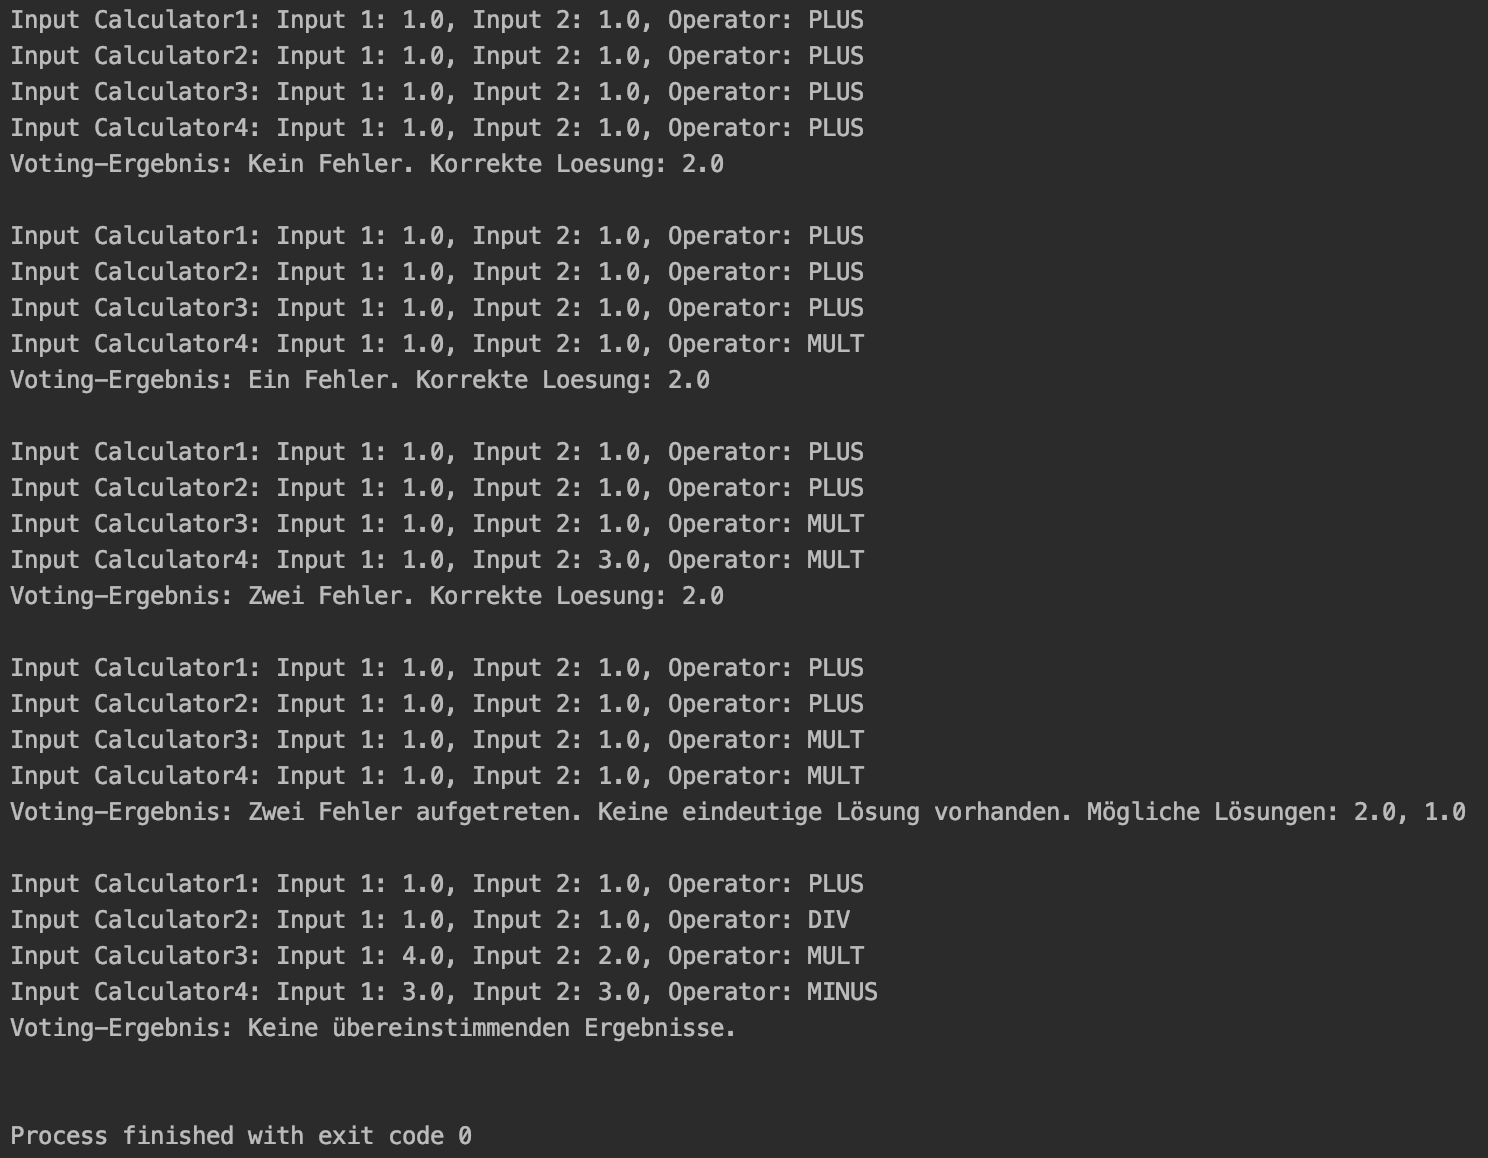
\includegraphics[width=1\textwidth]{images/tool_output.png}
\caption{Ausgabe des Tools}
\end{figure}